\section{Tomcat : conteneur de servlet Java EE}
%Nicolas
\subsection{Presentation}
\begin{frame}
  \frametitle{Présentation de Tomcat}

  \begin{itemize}
    \item Projet open-source de la fondation Apache
    \item Serveur d'applications Java
    \begin{itemize}
      \item Servlet (génération de page Html, xml etc...)
      \item JavaServer Pages
    \end{itemize}
    \item 
  \end{itemize}
\end{frame}

\begin{frame}
  \frametitle{Autres serveurs d'applications existants}
En réalité, Tomcat esseulement un conteneur de servlets, il existe des serveurs implémentant les normes JEE (sécurité, ejbs, transactions globales...) :
\begin{itemize} 
  \item GlassFish (D�veloppé par Oracle)
  \item jBoss (Utilise Tomcat pour la partie Servlet/JSP)
  \item Websphere (IBM)
  \item ...
\end{itemize}
\end{frame}

\begin{frame}
  \frametitle{Présentation Tomcat
  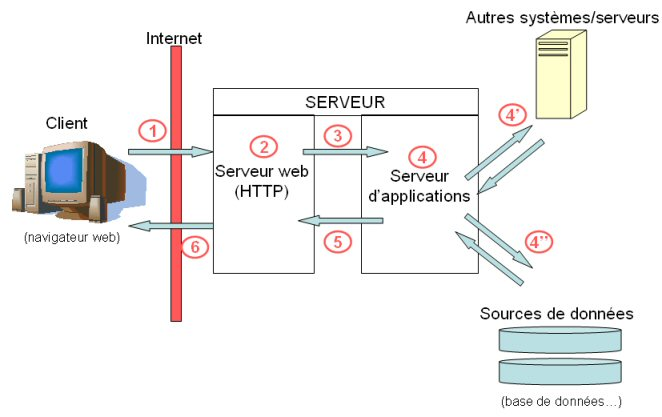
\includegraphics[scale=0.5]{Images/serveurapp.png}
\end{frame}

\subsection{Configuration}
\begin{frame}
  \frametitle{Fichiers de configuration}

		Répertoire d'installation : CATALINA\_HOME
\begin{itemize} 
    \item \textbf{bin/} exécutables de Tomcat(démarrage du serveur)
    \item \textbf{common/} classes et librairies partagées par les applications web
    \item \textbf{conf/} Fichiers de configuration
    \item \textbf{Logs/} Logs d'acc�s, erreurs...
    \item \textbf{server/} contient les applications web du serveur en lui-même
    \item \textbf{shared/} contient les classes et librairies partagées par toutes les applications web hébergées sur le serveur
    \item \textbf{temp/}
    \item \textbf{webapps/} contient les applications web
    \item \textbf{work/} contient les JSP compilée
\end{itemize} 
\end{frame}


\begin{frame}
  \frametitle{conf/server.xml}

\begin{itemize}
  \item \$CATALINA\_HOME/server.xml : principal fichier de configuration
  \item Eléments conteneurs (obligatoirs) : Engine, Host, Connector
  \item Définition des services, protocoles, port utilisés, redirection vers des ressources externes, des serveurs externes
  \item Eléments facultatifs : GlobalNamingResources, Resources, Realm et Valve.
\end{itemize} 

\begin{lstlisting}
  <Server port="8009" shutdown="SHUTDOWN">
  ...
  </Server>
\end{lstlisting}
		
}


\begin{frame}
  \frametitle{conf/server.xml}
		Eléments Connecteur
		\begin{itemize} 
   		\item objet Java capable d'écouter un port précis et comprenant un protocole pré
    	\item redirige les requêtes qu'il reçoit au moteur de servlets du servi
      \item C'est l'�l�ment qui re�oit les requ�tes HTTP et les transmet au conteneur de servlet
		\end{itemize}

		\begin{lstlisting}
<Connector port="8080"
	protocol="HTTP/1.1"
	connectionTimeout="20000"
	maxThread="100"
	maxCount="100"
	redirectPort="8443" />
		\end{lstlisting}
\end{frame}

\begin{frame}
    \frametitle{conf/server.xml}
		Eléments Engine et ost
		\begin{itemize}
   		\item \textbf{Elément Engine} : modélise le moteur de servlet, contient un ou plusies hosts
    	\item \textbf{ElémentHost} hôte virtuelSimilaire aux virtualhosts d'Apache)
		\end{itemize}

		\begin{lstlisting}
<Engine name="Catalina">
  <Host name="localhost" appBase="webapps"
    unpackWARs="true" autoDeploy="true">
    <!-- contenu de l'élément Host -->
  </Host>
</Engine>
		\end{lstlisting}
\end{frame}

\begin{frame}
  \frametitle{conf/server.xml}
		Resssources et variables d'environnement

		\begin{lstlisting}
<GlobalNamingResources>
  <Resource name="UserDatabase" auth="Container" type="org.apache.catalina.UserDatabase" description="User database that can be updated and saved" factory="org.apache.catalina.users.MemoryUserDatabaseFactory" pathname="conf/tomcat-users.xml" />
  <Environment name="maxRetry" type="java.lang.Integer" value="10" override="false"/>
</GlobalNamingResources>

		\end{lstlisting}
\end{frame}

\subsection{D�ploiement d'une application}
\begin{frame}
\frametitle{Via le manager}
	Installation d'une application web sous la forme d'une archive war
  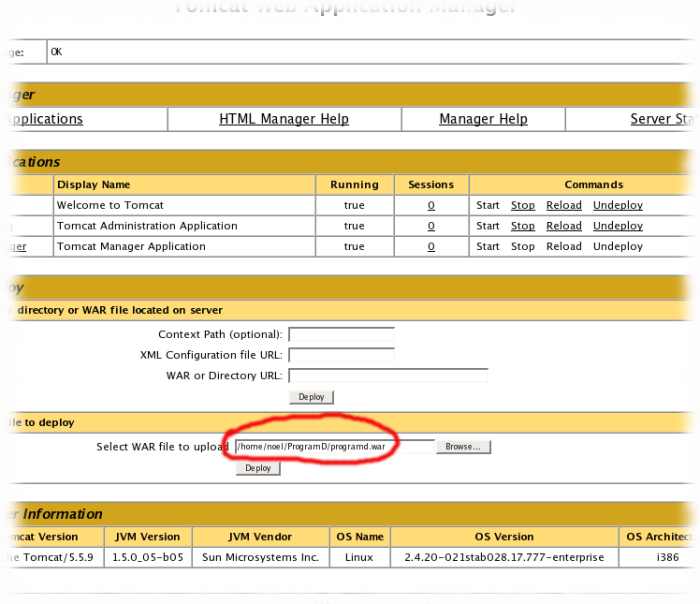
\includegraphics[scale=0.3]{Images/tomcat-deploy-war.png}
\end{frame}

\begin{frame}
  \frametitle{Directement dans le dossier de Tomcat}

  \begin{itemize}
    \item Placer l'archive war dans le dossier webapps/
    \item Tomcat d�compresse l'application au démarrage
    \item L'application est accessible par l'url http://serveur.tld/nom\_archive\_war
  \end{itemize}
\end{frame}

